\documentclass[10pt,a4paper]{scrartcl}

%\setkomafont{disposition}{\rmfamily}

\usepackage[utf8]{inputenc}
\usepackage{hyperref}
\usepackage{amssymb}
\usepackage{amsmath}
\usepackage{graphicx}
\usepackage{caption}
\usepackage{subcaption}
\usepackage{amsmath,amssymb,amsthm}

\usepackage{geometry}\geometry{a4paper,left=30mm,right=30mm,top=25mm,bottom=20mm}

\usepackage{tikz}

\usepackage[]{todonotes}  %% other options: colorinlistoftodos,prependcaption,textsize=tiny
\usepackage{bigfoot}

\begin{document}

\title{Report}
\subtitle{Study of RSE GitHub repositories}
\author{Kara Moraw}
\date{\today}
\maketitle

\section{Motivation}

We want to investigate how research software projects have changed over time, how they evolve and how they differ between disciplines by analysing relevant software repositories.
This will help us gain a better understanding of ongoing processes in the research software community and of how they can be supported.
It will also supply evidence about which practices aid to build and maintain software with a wider community engagement.

\subsection*{Hypothesis}

The following is not meant to be a fixed set of things we want to find, but rather some ideas that may help guide what data is worth collecting.
We hypothesise that
\begin{enumerate}
    \item research software repositories evolve in four stages
    \begin{enumerate}
        \item \textit{no engagement:} sparse commits, no issues, few authors, no license, no DOI citation
        \item \textit{publication:} DOI, license, usage guidelines, some watchers/stars, some issues created and resolved by repository maintainers
        \item \textit{low engagement:} external users create issues, maintainers resolve issues, forks
        \item \textit{community engagement:} external users create and resolve issues, merge requests
    \end{enumerate}
    \item research software repositories that employ good practices reach higher stages (earlier)
\end{enumerate}

Can we find markers that indicate transition into the next phase?

\section{Methods}

\subsection*{Data Collection}

\todo[inline]{Would need to add references to GitHub and other software used.}
In this study, we wanted to focus on software repositories created by RSEs for their research and collect a comprehensive set of metrics.
To find the respective repositories, we decided to scan a large set of publications available through ePrints repositories of UK universities.
As GitHub has been identified as the most commonly used software repository host\todo{Citation missing}, we look for links in the publication text that contain \verb|github.com|.
We then chose a subset of the repositories found this way and use the GitHub API to collect metrics about the repositories.

\subsubsection*{Scanning ePrints repositories}

We scanned a total of 211,602 PDF files from ePrints entries across 16 ePrints repositories. For details, see table \ref{table:eprints}.
For each repository, we used the advanced search feature to select papers published between 2010 and the date of analysis (June 2023). % filtered for pres_type=paper and date=2010-
If a PDF was available, we parsed it and looked for any links to GitHub using a low-fidelity regular expression.\footnote{\verb|(?P<url>https?://(www\.)?github\.com[^\s]+)|}

In this manner, we extracted a total of 2,391 links. Afterwards, we validated them against existing GitHub repositories:
\begin{enumerate}
    \item The links were matched against the standard GitHub URL pattern, where the domain is followed by a username and a repository name. This expression was also able to separate multiple links that had been detected as one expression before.\footnote{\verb|github\.com/[A-Za-z0-9-]+/[A-Za-z_\-]+|}
    \item Next, we used the GitHub API to check that the detected user owned a repository with a name similar enough to the detected one. Specifically, we matched it against the highest scoring existing repository with a Levenshtein distance to the detected name of at least $0.7$.
\end{enumerate}
This left a total of 1,975 unique links.
In the following data collection steps, we only used these validated GitHub URLs.

The resulting dataset is described in table \ref{table:github_eprints}.

\begin{table}
    \begin{tabular}{|l|l|}
        \hline
        Data attribute & description \\
        \hline 
        \verb|eprints_repo| & ePrints repository name\\
        \verb|title| & publication title\\
        \verb|author_for_reference| & one of the listed authors\\
        \verb|date| & date field for the ePrints entry of the publication\\
        \verb|year| & year extracted from date\\
        \verb|pdf_url| & URL of publication PDF\\
        \verb|page_no| & number of the page where the GitHub link was found\\
        \verb|domain_url| & GitHub link\\
        \verb|pattern_cleaned_url| & GitHub link after advanced regular expression matching\\
        \verb|github_user_cleaned_url| & matching existing repository on GitHub\\
        \hline
    \end{tabular}
    \caption{Schema for dataset of GitHub links in publications hosted in ePrints repositories.}
    \label{table:github_eprints}
\end{table}

\subsubsection*{Selection of relevant GitHub links}
\label{section:select_links}

Links to GitHub repositories can be included in a publication for multiple reasons:\todo{There are publications on this, cite one here.}
\begin{enumerate}
    \item The authors created the software or data in the repository as part of the work carried out for the publication.
    \item The authors used the software or data in the repository in their work for the publication, e.g. as a scientific tool or for visualisation.
    \item The repository is cited as related work.
\end{enumerate}

For this study, we were only interested in the first kind since we can be sure that the software was written by RSEs for research.
However, classifying a link with respect to the listed categories is non-trivial.\todo{Could add a citation here, check CZI Hackathon paper.}

After reviewing a few papers manually, we found that links on the first two pages of a publication often corresponded to references of the first type,
with authors providing a link at the end of the abstract or in a footnote linked to from the abstract or introduction.
A mapping of links to sections would yield a similar and possibly more accurate and informative heuristic,
but parsing sections requires more computational effort and is non-trivial for footnotes.
Hence, we decided to continue the analysis with only those repositories that had been linked on the first two pages.
We did not validate how many links of type 1 were found on later pages,
but would expect that methods sections would contain links of both types.

We manually reviewed the corresponding publications and annotated this set with the labels \textit{created} (type 1) and \textit{not created} (types 2 and 3).
Of the NUMBER repositories, we found NUMBER to be linked as software created as part of the work carried out for the publication.\todo{Fill in numbers.}

\subsubsection*{Metric collection via GitHub API}

For all repositories found on the first two pages, we used the GitHub API to collect a large set of data for each of the repositories:
\todo[inline]{List collected data.}

\begin{itemize}
    \item repository metadata
    \item repository contents (license, README, contributing guidelines, citation file)
    \item commit details
    \item issue details
    \item changes in README headings (file history)
    \item star and fork events
\end{itemize}

The data schemas are appended in appendix \ref{section:app_schemas_collection}.

\subsection*{Data Aggregation/Analysis?}

First, we added two labels to the repository metadata: \textit{license type} and \textit{readme size category}.
License type is one of \textit{permissive}, \textit{non-permissive}, \textit{unknown} and \textit{none} (no license detected)\footnote{More info about GitHub license recognition: \url{https://docs.github.com/en/rest/licenses/licenses?apiVersion=2022-11-28}}.
The following licenses are considered as \textit{permissive}: MIT, GPL-3.0, Apache-2.0, BSD-3-Clause, GPL-2.0 and BSD-3-Clause.
Any other recognised license is considered \textit{non-permissive}.
If the license is not recognised by GitHub (but there is one), it is categorised as unknown.
The mapping of licenses to types is listed in the appendix.\todo{add list of license to type, and reference - was that Wiki?}
The GitHub API provides the size of the README file in bytes.
Through empirical manual evaluation, we determined five categories for READMEs indicated by their length:
\begin{itemize}
    \item none: No README, byte size $0$.
    \item ultra-short: README file size is at least $1$ Byte but lower than $300$ Bytes. These are READMEs with only a title and a one-sentence description.
    \item short: At least $300$ Bytes but lower than $1500$. These are READMEs with a longer description or one section about e.g. how to run the software.
    \item informative: At least $1500$ Bytes but lower than $10,000$. Multiple sections covering e.g. requirements, installation and running instructions.
    \item detailed: Over $10,000$ Bytes. Extensive documentation including images and example use cases.
\end{itemize}

Our main interest is the lifecycle of a research software repository, so we aggregated the collected data into timelines
with respect to the age of the repository in weeks.

To this end, we first mapped out the occurrence of general events in terms of repository age, calculated from the event date obtained during data collection.
We considered the following events:
\begin{itemize}
    \item Ownership heading added: A commit to the README file included an addition to a headline with an ownership keyword (license, example, reference, citation, cited, publication, paper).
    \item Usage heading added: A commit to the README file included an addition to a headline with an ownership keyword (requirements, using, example, usage, run, install, tutorial, build, guide, documentation).
    \item Citation added: A commit to the README file included an addition to a line containing a citation indicator (\verb|DOI:|, \verb|doi.|, \verb|@article|, \verb|@misc|)
    \item Citation file added: A \verb|citation.cff| file was created.
    \item Contributing file added: A \verb|CONTRIBUTING.md| file was created.
    \item Paper published: A paper available in one of the ePrints repositories that contains a link to the repository is published (based on the \verb|date| field in ePrints).
\end{itemize}

The collected fork and star events were also reshaped to map to weeks since repository creation.

Finally, we created two user timeline datasets: one for contributing users (i.e. commit authors) and one for issue users.
Both contain one line for each week in the repository lifetime and each associated user, for all repositories.
For the contributing user timeline, we determine whether a user can be considered active in a specific week for a repository.
A user is considered active if they have made at least one commit in the last 12 weeks.
This is to account for pauses in development that might not mean that a contributor has left the team.
With this information, we can look at two aspects of team size over time:
The pool of active contributors, and the overall pool of contributors. 
As soon as a user makes a first commit, they become a member of both pools,
but they drop out of the active contributor pool after a phase of inactivity.

We add a similar label for issue users, namely the user status. This can be
\begin{itemize}
    \item inactive: the user has not been engaging with issues.
    \item opening: the user has opened at least one issue in the past 12 weeks.
    \item closing: the user has closed at least one issue in the past 12 weeks.
    \item both: the user has both the opening and closing status.
\end{itemize}

This process results in four output datasets:
\begin{enumerate}
    \item Metadata: One record per repository, containing metadata like the presence of a wiki, the license type, and the maximum observed number of active contributors in one week
    \item Weekly timeline containing events and trends: One record per week in the life of the repository, for each repository, indicating trends like the number of stars at that point in time and events like the addition of a citation file.
    \item Contributing user timeline: One record per each repository, user associated with the repository commit history and week in the life of the repository, indicating the user status.
    \item Issue user timeline: One record per each repository, user associated with the repository issues and week in the life of the repository, indicating the user status.
\end{enumerate}

The schemas for the datasets are appended in appendix \ref{section:app_schemas_output}.

\section{Limitations}
\label{section:limits}

The GitHub API includes pull requests in issues, so in our datasets, issues might be both.
We cannot distinguish the two in our dataset.

The contribution dataset only includes commits to the main branch and doesn't include commits that merge a pull request, neither for the user merging the PR nor for the users that contributed to the PR.
In our analysis, a good development workflow of opening a PR, committing to it, and merging it does not get picked up.

Finally, we interpret the date field extracted from ePrints as the publication date.
This might not always be correct as the definition for this field doesn't seem to explicitly relate to the publication,
and it is unclear whether it refers to the presentation at a conference, the publication of a preprint or the journal publication.
However, we expect it to be a good enough approximation. 

\section{Findings}
\todo[inline]{Not separating results and discussion yet, might consider doing so later.}

\begin{itemize}
    \item There are a few repos with high number of stars and decent number of forks that do not have any new contributors. None of the repos seem to use issues a lot, mostly for bug fixing (i.e. open shortly)? Maybe people are more inclined to contribute with a CONTRIBUTING file and some inviting tags like "good first issue" etc.
    \item ML repos might lead to higher engagement per default, I think (haven't validated) that the one-person repos with some engagement usually had to do with ML.
\end{itemize}

\subsection*{Software mentions}

\begin{figure}[h]
    \centering
    \begin{subfigure}[t]{0.3\textwidth}
        \centering
        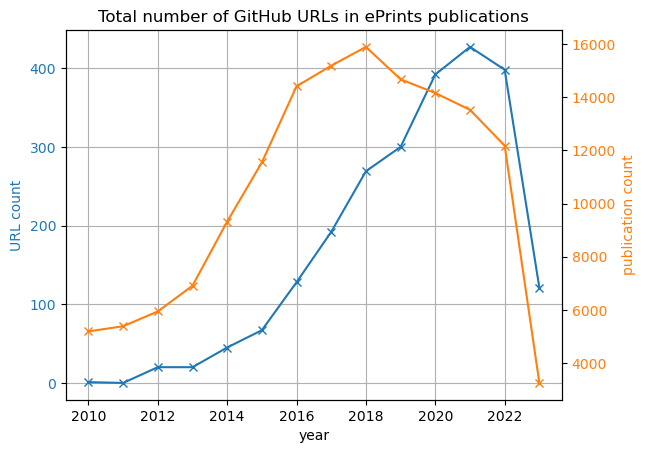
\includegraphics[width=\textwidth]{../analysis/overall/github_in_eprints.png}
        \caption{In blue, the number of GitHub links found across all publications per year. In orange, the number of publications.}
        \label{fig:gh_in_ep_no}
    \end{subfigure}
    \hfill
    \begin{subfigure}[t]{0.3\textwidth}
        \centering
        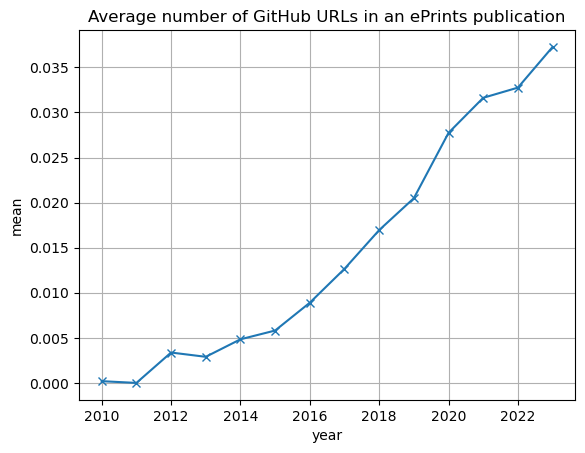
\includegraphics[width=\textwidth]{../analysis/overall/avg_github_in_eprints.png}
        \caption{Average number of GitHub links in one publication.}
        \label{fig:gh_ep_mean}
    \end{subfigure}
    \hfill
    \begin{subfigure}[t]{0.3\textwidth}
        \centering
        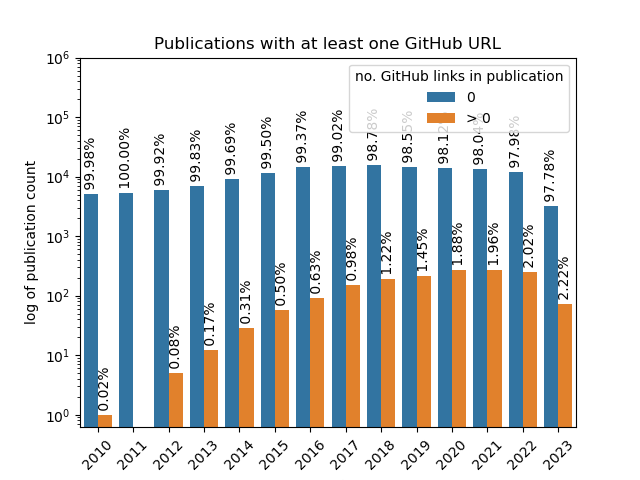
\includegraphics[width=\textwidth]{../analysis/overall/min_one_github_in_eprints.png}
        \caption{How many publications in a year contained at least one GitHub link.
        Those that did are displayed in orange bars, those that did not contain a single link are shown in blue bars.
        Note that the y-axis scales logarithmically.
        On top of the bars is the percentage of the total number of publications represented by the bar.}
        \label{fig:gh_ep_min_one}
    \end{subfigure}
       \caption{GitHub links in ePrints publications over time.}
       \label{fig:gh_ep}
\end{figure}

Figure \ref{fig:gh_ep} shows that even though the number of GitHub links included in ePrints publications is small,
it has steadily increased in the past 13 years.
The main driver could be that software becomes ever more important across a variety of research domains,
but the developments also indicate that referencing software code has become more common.

\subsection*{Mention type}

\begin{figure}[h]
    \centering
    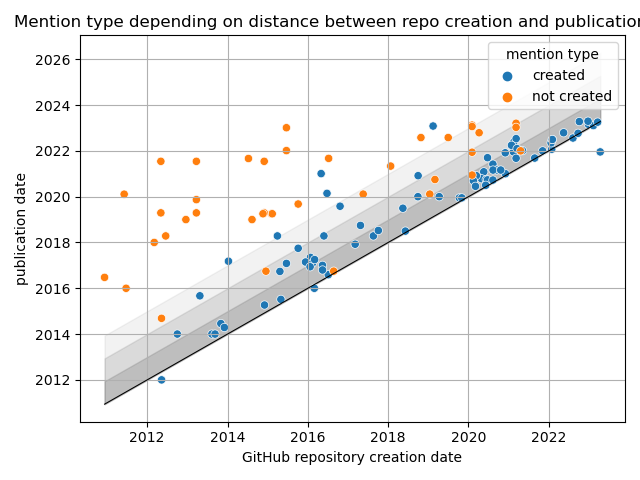
\includegraphics[width=0.5\textwidth]{../analysis/overall/mention_type_timeline.png}
    \caption{Mention type indicated by dot colour plotted against repository age at time of publication.}
    \label{fig:mention_type_time}
\end{figure}

As described in section \ref{section:select_links}, we manually annotated links found on the first two pages of a publication as \textit{created} or \textit{referenced}.
Figure \ref{fig:mention_type_time} shows that links for software that has been created three years before publication are usually references and not created as part of the publication.
Interestingly, from 2019 forward, links that are older than one year also tend to be references and not creations,
suggesting that the time between software being published and picked up on by the community might have shortened. 
From 2020 forward, a much larger portion of the software is of the \textit{created} type and published earlier (within a year),
indicating that researchers create and link their software more since then.
However, this analysis might be biased because a larger time span is available for older software.

\todo[inline]{Ideally, quantify these analyses instead of 'just' looking at the graph.}

The graph suggests that the age of the repository at time of publication could be used as
an indicator about how likely it is that the linked repository was created for this work or simply referenced.
It's not fit for use as a classifier though, since the threshold seems to change from three years to only one year over the years.

We also looked at classifying links as \textit{referenced} if they were detected more than once in the same publication.
This didn't prove to be a good indicator as we only found 10 duplicate links across the whole dataset, all of which were \textit{created}.

\subsection*{Overall analysis}

Ideas: \todo{implement some or remove}
\begin{itemize}
    \item adjust repo timelines to sort issue and contributor user plots by first date to make the visualisation more intuitive
    \item plot timelines together for high interest repos, or by category?
    \item contrasting analysis of interest-based categories, i.e. forks, stars
\end{itemize}

\todo{Almost no citations, and other works have mined GitHub for repos with a DOI...}

\begin{figure}[h]
    \centering
    \begin{subfigure}[t]{0.8\textwidth}
        \centering
        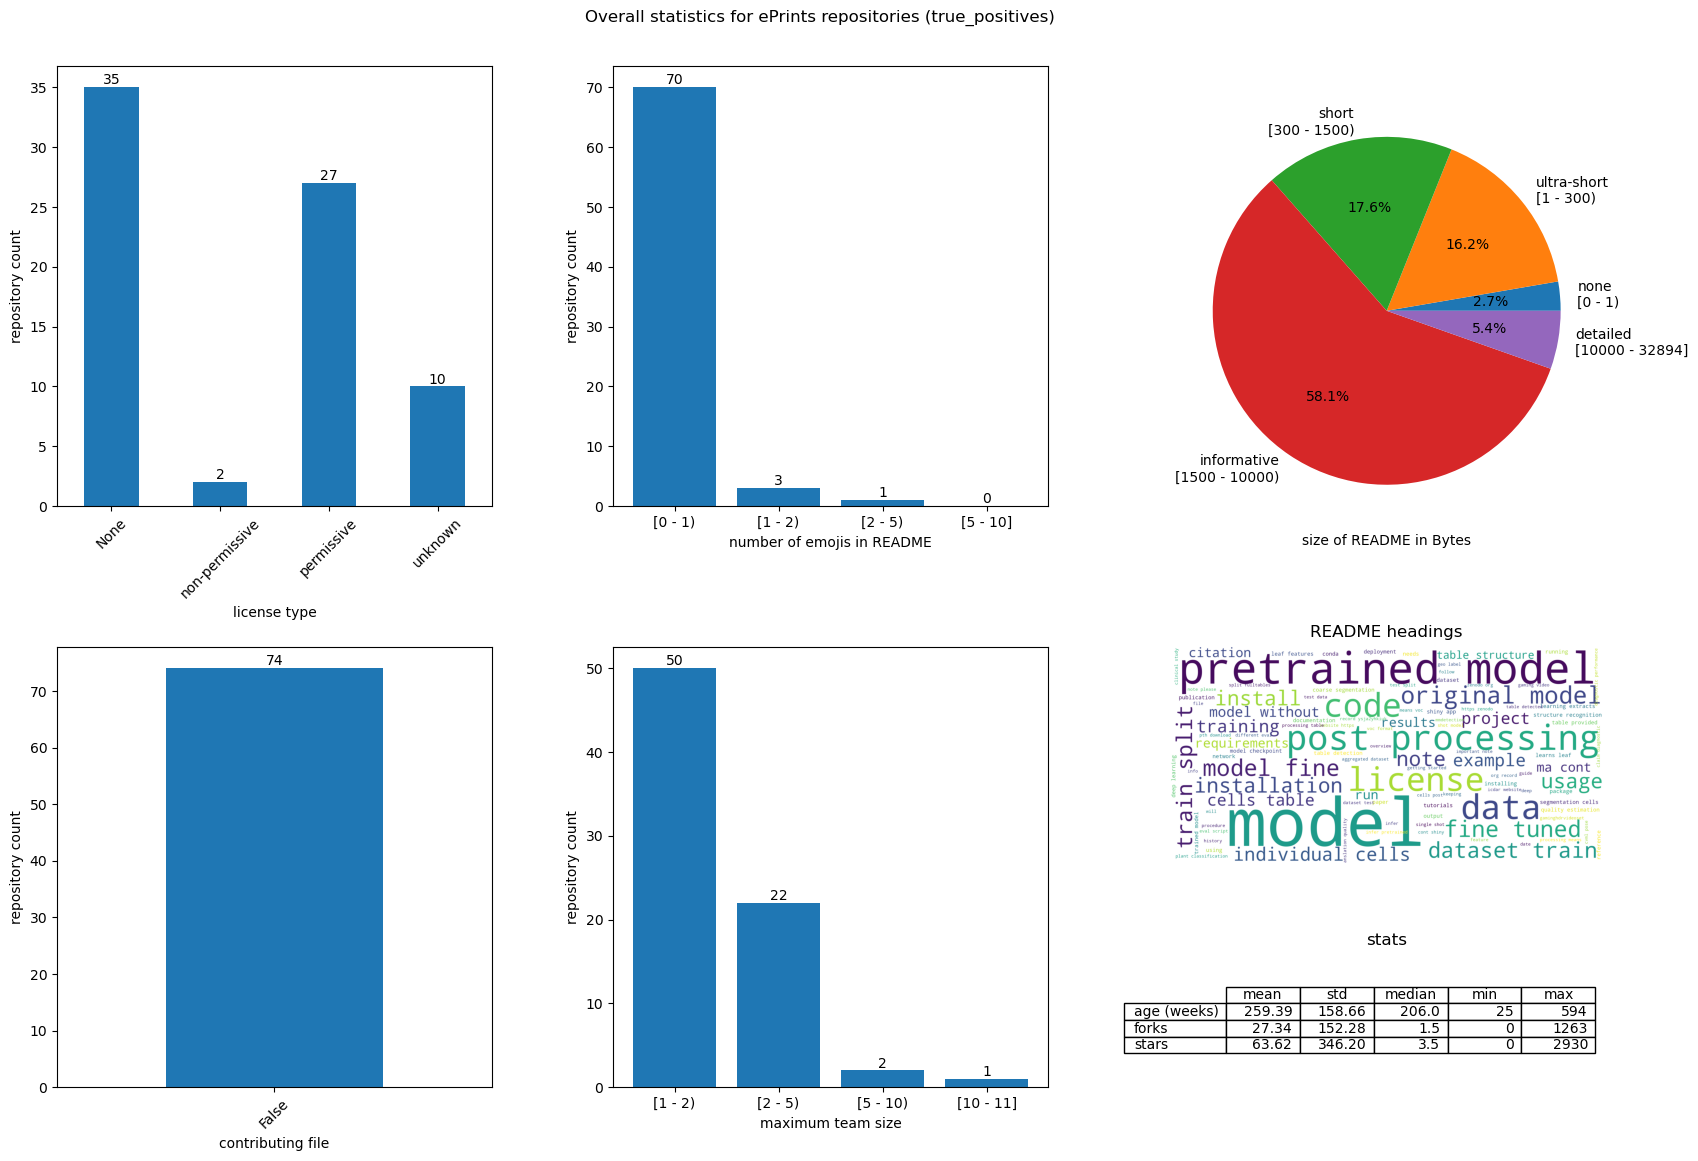
\includegraphics[width=\textwidth]{../analysis/overall/overall_true_positives.png}
        \caption{All repositories cited as created software.}
        \label{fig:overall_tp}
    \end{subfigure}\\
    \begin{subfigure}[t]{0.8\textwidth}
        \centering
        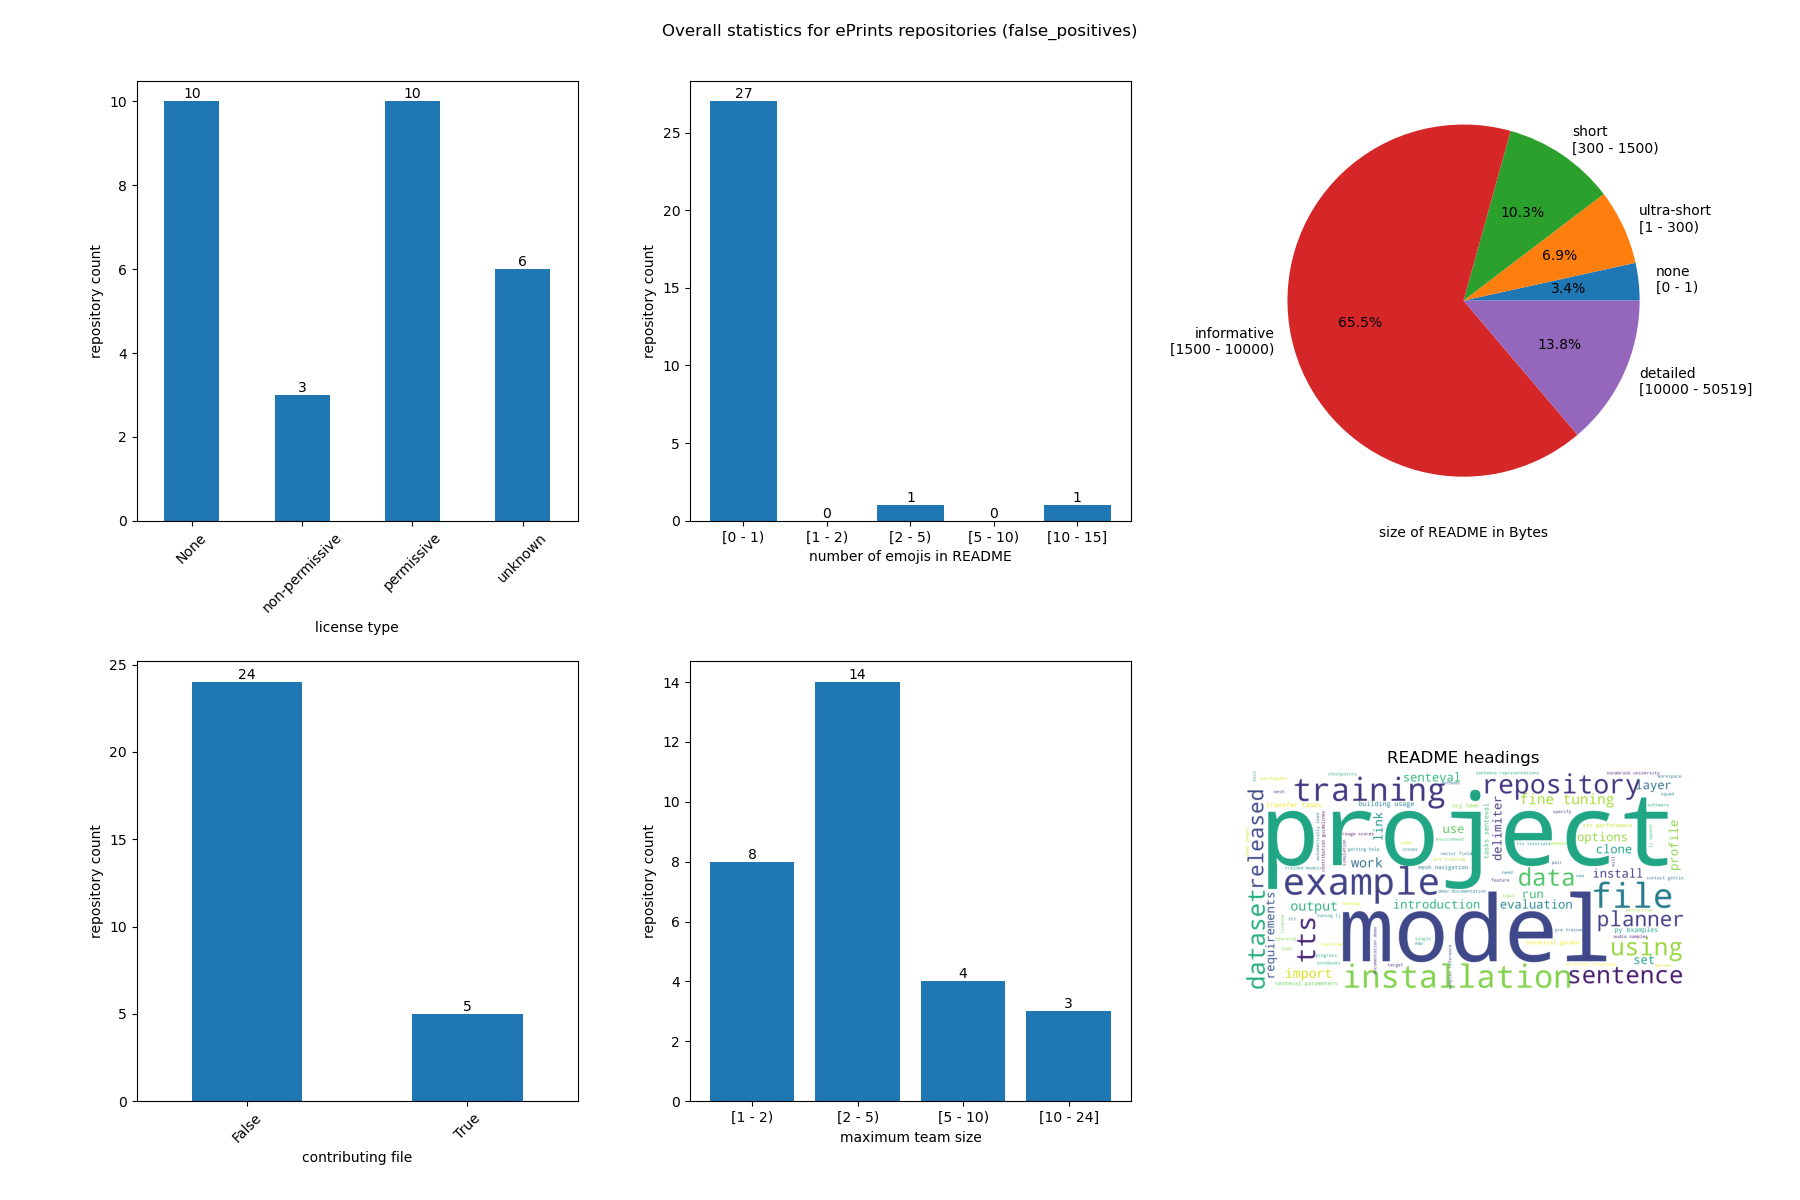
\includegraphics[width=\textwidth]{../analysis/overall/overall_false_positives.png}
        \caption{All repositories linked but not created for the publication.}
        \label{fig:overall_fp}
    \end{subfigure}
    \caption{Overall statistics.}
    \label{fig:overall_tfp}
\end{figure}

Figure \ref{fig:overall_tfp} compares different statistics between software repositories that have been mentioned as \textit{created} for the publication
and those that have been mentioned for other reasons.
The most notable difference is that there is a much higher proportion of repositories contributed to by only one user in the former.
Not surprisingly, the latter have a significantly higher median number of forks and stars and tend to be older,
indicating that software linked for reasons other than creation is usually popular.

Figure \ref{fig:overall_tp} shows that a worryingly high number of repositories is created and linked as part of a scientific publication
but does not contain a license.
Non-permissive licenses are uncommon, but having no license is in some ways worse.

\begin{figure}[h]
    \centering
    \begin{subfigure}[t]{0.8\textwidth}
        \centering
        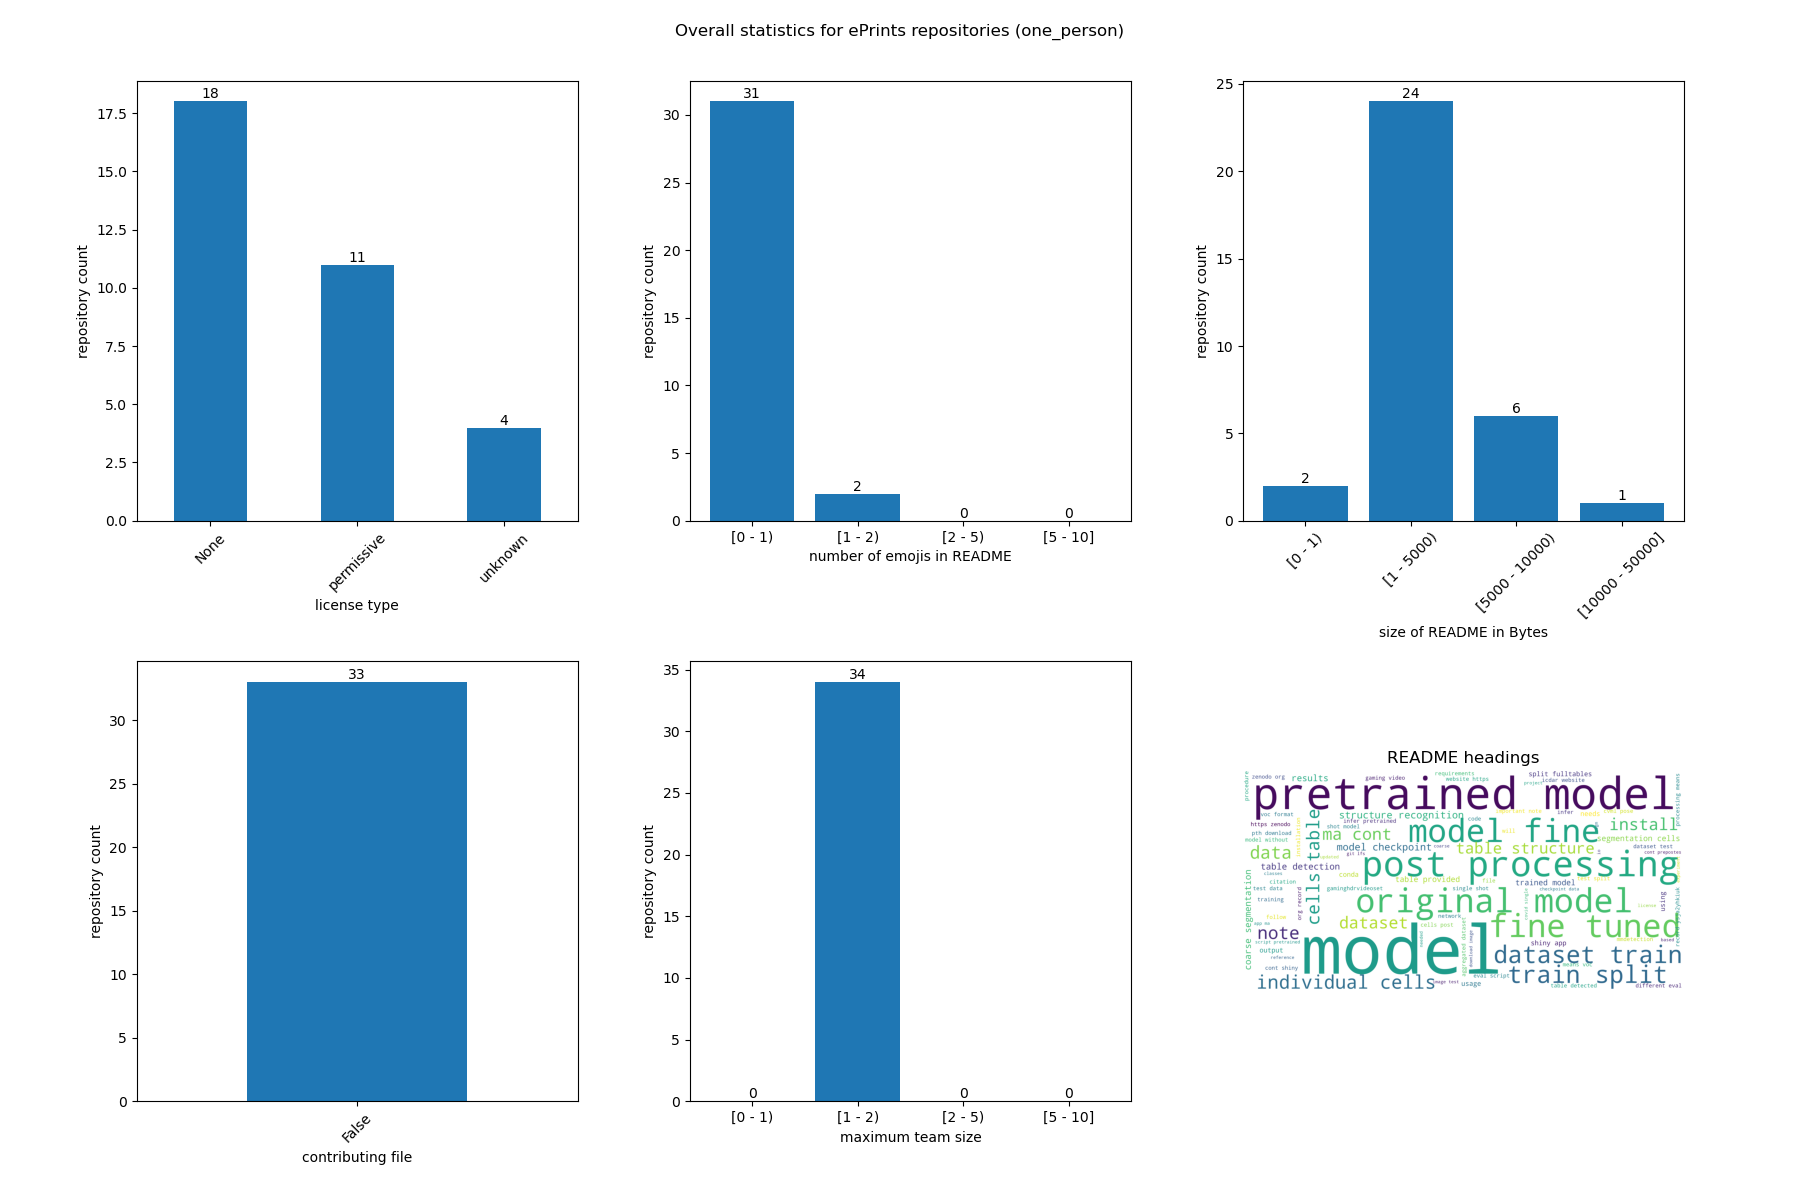
\includegraphics[width=\textwidth]{../analysis/overall/overall_one_person.png}
        \caption{One-person repositories.}
        \label{fig:overall_op}
    \end{subfigure}\\
    \begin{subfigure}[t]{0.8\textwidth}
        \centering
        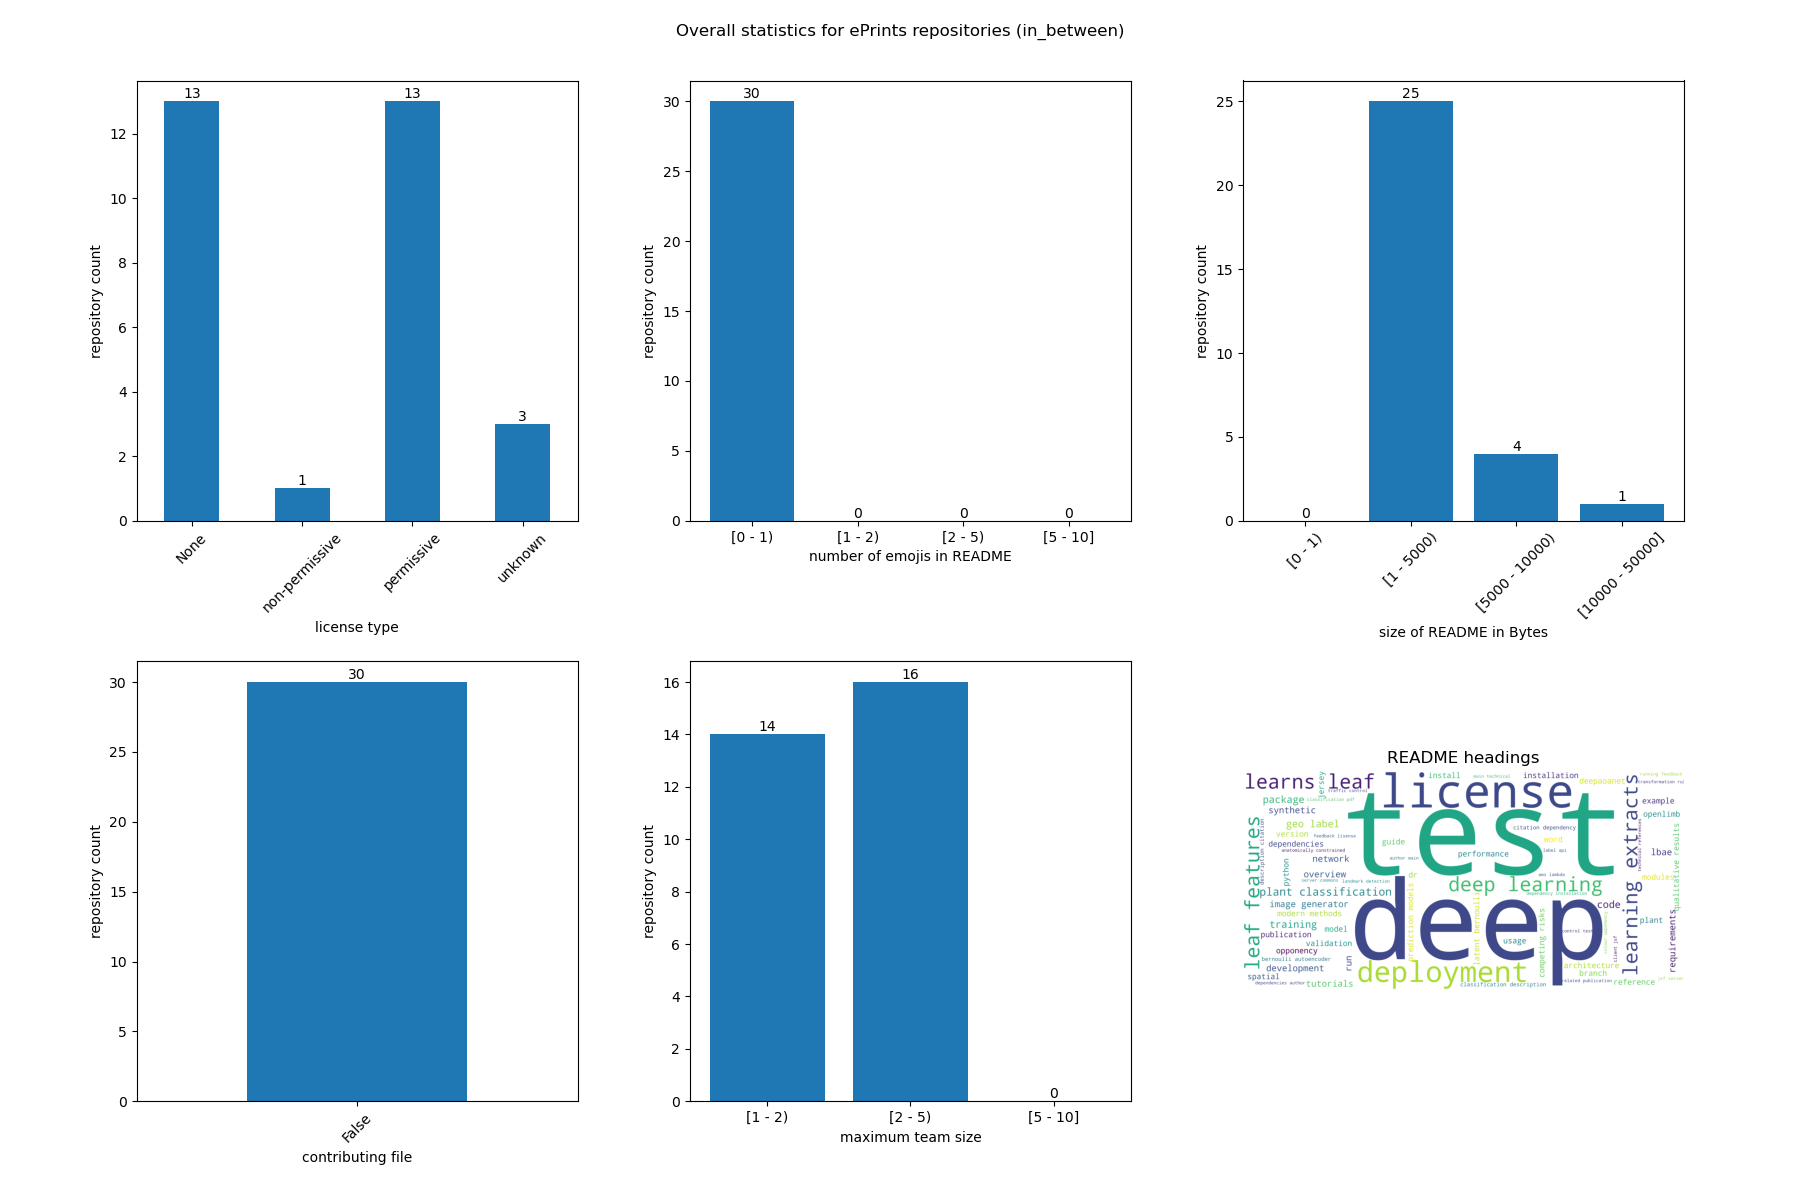
\includegraphics[width=\textwidth]{../analysis/overall/overall_in_between.png}
        \caption{In-between repositories.}
        \label{fig:overall_ib}
    \end{subfigure}\\
    \begin{subfigure}[t]{0.8\textwidth}
        \centering
        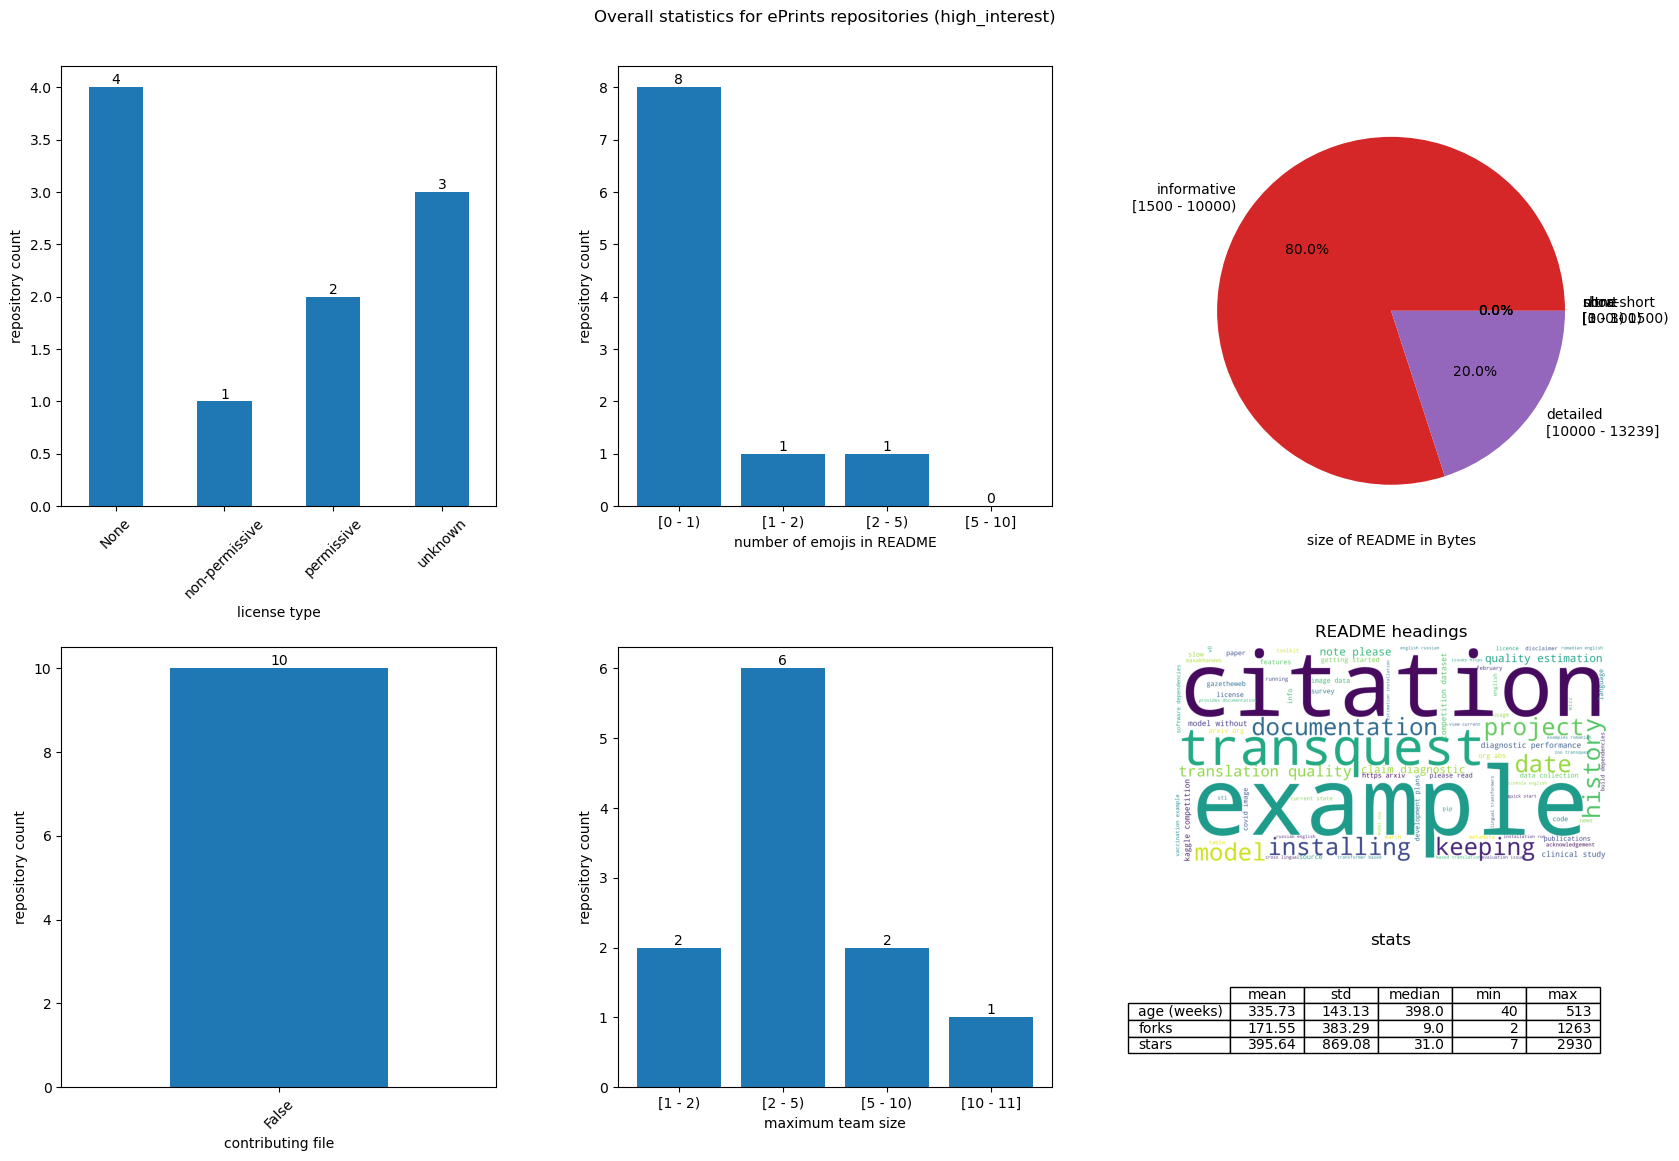
\includegraphics[width=\textwidth]{../analysis/overall/overall_high_interest.png}
        \caption{High-interest repositories.}
        \label{fig:overall_hi}
    \end{subfigure}
    \caption{Overall statistics.}
    \label{fig:overall_cats}
\end{figure}

In a next step, we manually assigned the repositories mentioned as \textit{created} one of three categories: \todo{rethink naming of categories ('interest' might not be ideal)}
\begin{enumerate}
    \item one-person repository (only one user interacts with issues and commits)
    \item high-interest repository (more than five users interact with issues and commits) \todo{check that this definition still matches...}
    \item in-between repository
\end{enumerate}
Figure \ref{fig:overall_cats} shows some notable differences between the three categories, for example that
high-interest repositories have no short README files.
Possibly, repositories with longer and thus more informative README files are easier for a wider community to interact with.
On the other hand, a repository with multiple users might evolve into having a longer, more informative README file
as multiple users need to become familiar with the software and keep up to date with any changes.

Moreover,  'test' emerges as a frequent README heading in in-between repositories
in contrast to one-person repositories,
and 'citation' is more frequently used in README headings high-interest repositories.
Again, it is less clear whether these are sections that are added to the README because of an increased user base,
or whether READMEs with these headings provide better support for a growing community.

Looking at the timeline graphs\todo{include timeline graphs or move this elsewhere},
it is evident that the owners of one-person repositories tend not to use issues for their own development.
This could be a reason for the non-existing interaction with other users:
there are no structures in place to make contributing straightforward,
and no indication about features currently in development.

\subsection*{Patterns}

The main pattern seems to be 
\begin{enumerate}
    \item Publication
    \item Interest
    \item Dormant
\end{enumerate}
with some variations in terms of magnitude.\todo{Add some timeline plots?}

For example, in one-person repos the interest only shows as stars.
They go dormant quicker than the others.
High-interest repositories keep interest for longer,
and it takes a different form, i.e. forks, PRs contributions (see for example \verb|GazeTheWeb|). 
Still, they go quiet after a while,
meaning that the number of active contributors goes down and there is less fluctuation in the number of issues. 
An exception is the repository \verb|nilmtk| which experiences interest in phases, i.e. not growth in interest,
but decreasing interest followed by again increased interest with newer contributors.

In \verb|esbmc|, we can observe two phases of interest after publication:
One where the contributor pool grows slowly and then one where it grows much quicker.

Mentions in publications later on (probably as related work or tool instead of "original work")
often lead to a spike in stars, sometimes even in forks.

The number of forks grows with the number of stars at a lower rate.
One exception is \verb|dissect-cf|, where the number of forks is larger than that of stars.

There are also a handful of repositories with apparently highly responsive owners
(e.g. \verb|Dusty-evolved-starkit| and \verb|transquest|).
Many issues are opened, but all are resolved by the owner so the contributing team does not grow.
However, these issues could all be pull requests (see notes on limitations in section \ref{section:limits}).

People who open issues and fork at the same time are usually adding a PR.
These people can become contributors, i.e. make commits to the main branch.
They don't do that when they are not interacted with though, meaning that their issues are left open.
One example of this is \verb|MOEADr|, where issues aren't responded to and PRs aren't commented on.

\subsection*{Case studies}

See timelines in \ref{fig:repo_timelines}.\todo{choose fewer, write more?}

\begin{itemize}
    \item \verb|ethanwharris/foveated-convolutions|: many stars
    \item \verb|gamesbyangelina/danesh|: stars increase at second publication, is this usage or creation?
    \item \verb|lphowell/GeothermalModelling|: three publications, what does this say about usage?
    \item \verb|philgooch/BADREX-Biomedical-Abbreviation-Expander|: informative README and license, stars, but still no contributors
    \item \verb|IraKorshunova/folk-rnn|
    \item \verb|MAMEN/GazeTheWeb|: example of ebb at the end, look into README headings?
    \item \verb|morriscb/The-wiZZ|: new contributor? what made this accessible?
    \item \verb|tharindudr/transquest|: only owner contributes
    \item \verb|fcampelo/MOEADr|: few contributors but loads of issue users
    \item \verb|intelaligent/tctb|
\end{itemize}

\begin{figure}[h]
    \centering
    \begin{subfigure}[t]{0.8\textwidth}
        \centering
        \includegraphics[width=\textwidth]{../analysis/repo_timelines/true_positives/one_user/ethanwharris-foveated-convolutions.png}
        \caption{ethanwharris/foveated-convolutions}
    \end{subfigure}\\
    \begin{subfigure}[t]{0.8\textwidth}
        \centering
        \includegraphics[width=\textwidth]{../analysis/repo_timelines/true_positives/one_user/gamesbyangelina-danesh.png}
        \caption{gamesbyangelina/danesh}
    \end{subfigure}\\
\end{figure}
\begin{figure}[h]\ContinuedFloat
    \centering
    \begin{subfigure}[t]{0.8\textwidth}
        \centering
        \includegraphics[width=\textwidth]{../analysis/repo_timelines/true_positives/one_user/lphowell-Geothermal-Modelling.png}
        \caption{lphowell/GeothermalModelling}
    \end{subfigure}\\
    \begin{subfigure}[t]{0.8\textwidth}
        \centering
        \includegraphics[width=\textwidth]{../analysis/repo_timelines/true_positives/one_user/philgooch-BADREX-Biomedical-Abbreviation-Expander.png}
        \caption{philgooch/BADREX-Biomedical-Abbreviation-Expander}
    \end{subfigure}\\
\end{figure}
\begin{figure}[h]\ContinuedFloat
    \centering
    \begin{subfigure}[t]{0.8\textwidth}
        \centering
        \includegraphics[width=\textwidth]{../analysis/repo_timelines/true_positives/many_users/IraKorshunova-folk-rnn.png}
        \caption{IraKorshunova/folk-rnn}
    \end{subfigure}\\
    \begin{subfigure}[t]{0.8\textwidth}
        \centering
        \includegraphics[width=\textwidth]{../analysis/repo_timelines/true_positives/many_users/MAMEM-GazeTheWeb.png}
        \caption{MAMEN/GazeTheWeb}
    \end{subfigure}\\
\end{figure}
\begin{figure}[h]\ContinuedFloat
    \centering
    \begin{subfigure}[t]{0.8\textwidth}
        \centering
        \includegraphics[width=\textwidth]{../analysis/repo_timelines/true_positives/many_users/morriscb-The-wiZZ.png}
        \caption{morriscb/The-wiZZ}
    \end{subfigure}\\
    \begin{subfigure}[t]{0.8\textwidth}
        \centering
        \includegraphics[width=\textwidth]{../analysis/repo_timelines/true_positives/many_users/tharindudr-transquest.png}
        \caption{tharindudr/transquest}
    \end{subfigure}\\
\end{figure}
\begin{figure}[h]\ContinuedFloat
    \centering
    \begin{subfigure}[t]{0.8\textwidth}
        \centering
        \includegraphics[width=\textwidth]{../analysis/repo_timelines/true_positives/inbetween/fcampelo-MOEADr.png}
        \caption{fcampelo/MOEADr}
    \end{subfigure}\\
    \begin{subfigure}[t]{0.8\textwidth}
        \centering
        \includegraphics[width=\textwidth]{../analysis/repo_timelines/true_positives/inbetween/intelaligent-tctb.png}
        \caption{intelaligent/tctb}
    \end{subfigure}\\
    \caption{Repository timelines.}
    \label{fig:repo_timelines}
\end{figure}

\section{Future?}

\begin{itemize}
    \item highlight analysis based on aggregated dataset
    \begin{itemize}
        \item does this relate to any of our research questions?
        \item for one-person repos it might shed light on what's missing or what they had but didn't make a difference
    \end{itemize}
    \item journal affiliation
    \item Pick out some repos (e.g. the ones mentioned as examples and a couple more) and draw the phases on them. Look at the length and start of those phases in terms of weeks: When do new contributors arrive? When does the repository go dormant?
    \item Differentiate between inactive forks, active forks that opened a PR and active forks that didn't open a PR.
    \item Does it help if the repository used issues from the beginning? I feel like most of the repos didn't do that, issues are start being opened once other people start engaging with the project.
    \item Does it help to respond to people's issues and close them?
    \item Are new people more likely to open issues if at publication date some issues had already been opened?
    \item could calculate timelines of CHAOSS metrics as indicators? Should have a good basis with the data we have collected and aggregated.
\end{itemize}

%\bibliographystyle{plain}
%\bibliography{literature}

\appendix

\section{Data collection details}

\todo[inline]{Fill this table, see GitHub issue.}
\begin{table}[h]
    \centering
    \begin{tabular}{|l|r|r|r|}
        \hline
        ePrints repository & number of publication files & number of PDFs & unique GitHub links \\
        \hline
        clok.uclan.ac.uk & 98,206 & 23,966 & 96 \\
        eprints.glos.ac.uk & 31,842 & 7,751 & 27 \\
        eprints.keele.ac.uk & 58,095 & 8,852 & 197 \\
        eprints.kingston.ac.uk & 36,071 & 6,326 & 43 \\
        eprints.lincoln.ac.uk & 84,336 & 13,278 & 191 \\
        eprints.nottingham.ac.uk & 107,501 & 21,615 & 129 \\
        eprints.soton.ac.uk & 7,317 & 6,488 & 140 \\
        eprints.worc.ac.uk & 22,062 & 3,569 & 21 \\
        irep.ntu.ac.uk & 74,071 & 12,180 & 148 \\
        openaccess.city.ac.uk & 127,146 & 38,083 & 292 \\
        publications.aston.ac.uk & 51,830 & 12,071 & 199 \\
        ray.yorksj.ac.uk & 18,951 & 4,789 & 11 \\
        repository.falmouth.ac.uk & 16,958 & 1,442 & 13 \\
        researchonline.ljmu.ac.uk & 81,066 & 25,444 & 348 \\
        researchspace.bathspa.ac.uk & 13,657 & 1,679 & 15 \\
        shura.shu.ac.uk & 93,101 & 24,069 & 105 \\
        
        \hline
        Total & 922,210 & 211,602 & 1,975\\
        \hline
    \end{tabular}
    \caption{Number of analysed ePrints entries. Files associated with an ePrints entry for an application can take a number of formats, including PDF, DOCX or JPEG.}
    \label{table:eprints}
\end{table}

\subsection*{Schemas}
\label{section:app_schemas_collection}

\todo{Add data type to schema... Not really a schema o/w.}

\begin{table}
    \centering
    \begin{tabular}{l|l}
        \hline
        Data attribute & Description \\
        \hline
        \verb|github_user_cleaned_url| & repository ID (format \verb|<user>/<repo_name>|) \\
        \verb|archived| & whether the repository is archived \\
        \verb|created_at| & date of repository creation \\
        \verb|has_wiki| & whether the repository has a wiki \\
        \verb|has_pages| & whether the repository has GitHub pages \\
        \hline
    \end{tabular}
    \caption{Schema for dataset of GitHub repository metadata.}
    \label{table:metadata}
\end{table}

\begin{table}
    \centering
    \begin{tabular}{l|l}
        \hline
        Data attribute & Description \\
        \hline
        \verb|github_user_cleaned_url| & repository ID (format \verb|<user>/<repo_name>|) \\
        \verb|license| & license type as recognised by GitHub API \\
        \verb|readme_size| & byte size of README file \\
        \verb|readme_path| & path to README file (usually \verb|./README.md|) \\
        \verb|readme_emojis| & number of emojis used in the README file \\
        \verb|contributing_size| & size of \verb|CONTRIBUTING.md| \\
        \verb|citation_added| & date that a \verb|CITATION.cff| file was added \\
        \verb|contributing_added| & date that a \verb|CONTRIBUTING.md| file was added \\
        \hline
    \end{tabular}
    \caption{Schema for dataset of GitHub repository contents.}
    \label{table:contents}
\end{table}

\begin{table}
    \centering
    \begin{tabular}{l|l}
        \hline
        Data attribute & Description \\
        \hline
        \verb|github_user_cleaned_url| & repository ID (format \verb|<user>/<repo_name>|) \\
        \verb|author| & user ID of commit author \\
        \verb|week_co| & date of start a week \\
        \verb|commits| & number of commits the author made in that week \\
        \hline
    \end{tabular}
    \caption{Schema for dataset of GitHub repository contributions.}
    \label{table:contributions}
\end{table}

\begin{table}
    \centering
    \begin{tabular}{l|l}
        \hline
        Data attribute & Description \\
        \hline
        \verb|github_user_cleaned_url| & repository ID (format \verb|<user>/<repo_name>|) \\
        \verb|state| & issue state at date of crawling (June 2023) \\
        \verb|created_at| & date of issue creation \\
        \verb|user| & user ID of issue author \\
        \verb|closed_at| & date the issue was closed (can be empty) \\
        \verb|closed_by| & user ID of user who closed the issue (can be empty) \\
        \hline
    \end{tabular}
    \caption{Schema for dataset of GitHub repository issues.}
    \label{table:issues}
\end{table}

\begin{table}
    \centering
    \begin{tabular}{l|l}
        \hline
        Data attribute & Description \\
        \hline
        \verb|github_user_cleaned_url| & repository ID (format \verb|<user>/<repo_name>|) \\
        \verb|readme_path| & path to README file (usually \verb|./README.md|) \\
        \verb|author_date| & date of commit to README \\
        \verb|added_headings| & new headings \\
        \verb|deleted_headings| & removed headings \\
        \verb|added_cites| & new citation info (DOI etc.) \\
        \hline
    \end{tabular}
    \caption{Schema for dataset of GitHub repository README file history, considering only changes to headings. Note that only headings beginning with \texttt{\#} are parsed, not those with \texttt{===} underneath.}
    \label{table:readme_headings}
\end{table}

\begin{table}
    \centering
    \begin{tabular}{l|l}
        \hline
        Data attribute & Description \\
        \hline
        \verb|github_user_cleaned_url| & repository ID (format \verb|<user>/<repo_name>|) \\
        \verb|date| & date of star \\
        \verb|user| & user ID of user that starred the repository \\
        \hline
    \end{tabular}
    \caption{Schema for dataset of GitHub repository star events.}
    \label{table:stars}
\end{table}

\begin{table}
    \centering
    \begin{tabular}{l|l}
        \hline
        Data attribute & Description \\
        \hline
        \verb|github_user_cleaned_url| & repository ID (format \verb|<user>/<repo_name>|) \\
        \verb|date| & date of fork \\
        \verb|user| & user ID of user that forked the repository \\
        \hline
    \end{tabular}
    \caption{Schema for dataset of GitHub repository fork events.}
    \label{table:forks}
\end{table}

\section{Schemas for output datasets}
\label{section:app_schemas_output}

\todo{Add data type to schema... Not really a schema o/w.}

\begin{table}
    \centering
    \begin{tabular}{|l|l|}
        \hline
        Data attribute & Description \\
        \hline
        \verb|github_user_cleaned_url| & repository ID (format \verb|<user>/<repo_name>|) \\
        \verb|archived| & whether the repository is archived \\
        \verb|created_at| & date of repository creation \\
        \verb|has_wiki| & whether the repository has a wiki \\
        \verb|has_pages| & whether the repository has GitHub pages \\
        \verb|license| & license type as recognised by GitHub API \\
        \verb|readme_size| & byte size of README file \\
        \verb|readme_path| & path to README file (usually \verb|./README.md|) \\
        \verb|readme_emojis| & number of emojis used in the README file \\
        \verb|contributing_size| & size of \verb|CONTRIBUTING.md| \\
        \verb|citation_added| & date that a \verb|CITATION.cff| file was added \\
        \verb|contributing_added| & date that a \verb|CONTRIBUTING.md| file was added \\
        \verb|week_since_repo_creation_citation_added| & number of weeks since creation of the repository when a citation file was first added.\\
        \verb|week_since_repo_creation_contributing_added| & number of weeks since creation of the repository when contributing guidelines were first added.\\
        \verb|license_type| & permissive, non-permissive, unknown or None\\
        \verb|readme_size_class| & categorisation of the README size based on the size in bytes (classes were determined empirically). One of ultra-short, short, informative, detailed.\\
        \verb|forks_count| & number of forks the repository had at date of analysis (June 2023) \\
        \verb|stars_count| & number of stars the repository had at date of analysis (June 2023) \\
        \verb|max_active_contributors| & maximum number of contributors considered active at the same time \\
        \hline
    \end{tabular}
    \caption{Schema for dataset of aggregated overall information.}
    \label{table:schema_agg_overall}
\end{table}

\begin{table}
    \centering
    \begin{tabular}{|l|l|}
        \hline
        Data attribute & Description \\
        \hline
        \verb|github_user_cleaned_url| & repository ID (format \verb|<user>/<repo_name>|) \\
        \verb|week_since_repo_creation| & running week number for each week in the life of each repository (from creation until date of analysis) \\
        \verb|closed_count| & number of closed issues in that week for that repository \\
        \verb|open_count| & number of open issues in that week for that repository \\
        \verb|active_contributors| & number of active contributors in that week for that repository \\
        \verb|contributors| & number of contributors so far (includes inactive) \\
        \verb|forks_count| & number of forks in that week for that repository \\
        \verb|stars_count| & number of stars in that week for that repository \\
        \verb|ownership_added| & whether a heading with an ownership keyword was added in that week for that repository \\
        \verb|usage_added| & whether a heading with a usage keyword was added in that week for that repository \\
        \verb|citation_added| & whether a citation keyword was added to the README in that week for that repository \\
        \verb|citation_file_added| & whether a citation file was added in that week for that repository\\
        \verb|contributing_file_added| & whether contributing guidelines were added in that week for that repository \\
        \verb|paper_published| & whether a paper linking to this repository was published in that week for that repository \\
        \hline
    \end{tabular}
    \caption{Schema for dataset of aggregated timelines.}
    \label{table:schema_agg_timelines}
\end{table}

\begin{table}
    \centering
    \begin{tabular}{|l|l|}
        \hline
        Data attribute & Description \\
        \hline
        \verb|github_user_cleaned_url| & repository ID (format \verb|<user>/<repo_name>|) \\
        \verb|author| & user ID of commit author \\
        \verb|week_since_repo_creation| & running week number for each week in the life of each repository (from creation until date of analysis) \\
        \verb|commits| & number of commits made by the user that week to this repository \\
        \verb|active_contributors| & whether the user is considered an active contributor that week \\
        \hline
    \end{tabular}
    \caption{Schema for dataset of aggregated commit author timelines.}
    \label{table:schema_agg_commit_author}
\end{table}

\begin{table}
    \centering
    \begin{tabular}{|l|l|}
        \hline
        Data attribute & Description \\
        \hline
        \verb|github_user_cleaned_url| & repository ID (format \verb|<user>/<repo_name>|) \\
        \verb|week_since_repo_creation| & running week number for each week in the life of each repository (from creation until date of analysis) \\
        \verb|user| & user ID of someone interacting with issues \\
        \verb|created_count| & number of issues created by that user that week for that repository \\
        \verb|closed_count| & number of issues closed by that user that week for that repository \\
        \verb|user_status| & whether the user is inactive, opening issues, closing issues or both opening and closing issues \\
        \hline
    \end{tabular}
    \caption{Schema for dataset of aggregated issue user timelines.}
    \label{table:schema_agg_issue_users}
\end{table}

\end{document}
